\documentclass[12pt,a4paper]{article}
\usepackage[utf8]{inputenc}
\usepackage[german]{babel}
\usepackage[T1]{fontenc}
\usepackage{amsmath}
\usepackage{amsfonts}
\usepackage{amssymb}
\usepackage{graphicx}
\usepackage{float}
\usepackage[left=2cm,right=2cm,top=2cm,bottom=2cm]{geometry}
\author{Tim}

\begin{document}
\newpage
\tableofcontents
\newpage

\section{Versuchsbeschreibung}
Ziel des Versuches ist die Vermessung der Dampfdruckkurve und die Bestimmung der Verdampfungsenthalpie von Wasser.\\

\subsection{Dampfdruckkurve}
In diesem Versuch soll nur der Übergang zwischen dem flüssigen und gasförmigen Aggregatzustand betrachtet werden. \\
In einer Flüssigkeit in einem evakuiertem, abgeschlossenem Gefäß verdampfen und kondensieren die Moleküle bis sich ein Gleichgewicht einstellt. Der Druck des Dampfes ist von der Temperatur und der Flüssigkeit abhängig und wird als Dampfdruck oder Sättigungsdruck bezeichnet. Der Zusammenhang von Sättigungsdampfdruck und Temperatur wird als Dampfdruckkurve bezeichnet. Wäre das Gefäß nicht evakuiert, würde sich das Gleichgewicht langsamer einstellen, der Dampfdruck wäre allerdings der gleiche, da die Partialdrücke einzelner Gase von der Anwesenheit anderer Gase nicht beeinflusst werden.

\subsection{Verdampfungsenthalpie}
Die Verdampfungsenthalpie beschreibt, wie viel Energie notwendig ist, um ein Mol des jeweiligen Stoffs (in diesem Fall Wasser) zu Verdampfen. Führt man einer gewissen Menge flüssigem Wasser langsam immer mehr Wärmeenergie zu und misst dabei die Temperatur, so ist die Verdampfungsenthalpie als Plateau beobachtbar. Trotz des Zuführens weiterer Wärmeenergie ändert sich die Temperatur nicht. \\

Der Sättigungsdampfdruck wird quantitativ durch die Clausius-Clapeyron-Gleichung beim Phasenübergang flüssig-gasförmig beschrieben.

\begin{equation}
\frac{dp}{dT}=\frac{\nu \Lambda}{T(V_{gas}-			V_{flüssig})}
\end{equation}

Da $V_{gas} >> V_{flüssig}$ folgt unter der Annahme das sich die Verdampfungsenthalpie $\Lambda$ innerhalb von kleinen Temperaturbereichen nicht ändert mittels Integration den für diesen Versuch entscheidenden Zusammenhang:

\begin{equation}
\ln{(p/p_0)}=-\frac{\Lambda}{R} \left(\frac{1}{T}-			\frac{1}{T_0}\right)
\end{equation}

Mit diesem Zusammenhang kann die Verdampfungsenthalpie $\Lambda$ für verschiedene Temperaturen bestimmt werden, indem um diese Punkte innerhalb kleiner Temperaturänderungen eine Gerade angepasst wird.

\section{Aufbau und Durchführung}
\label{sec:Aufbau und Durchfühung}
\begin{figure}[H]
\includegraphics[width=\linewidth]{Bilder/AufbauB}
\caption[AufbauB]{Aufbau}
\label{fig:AufbauB}
\end{figure}

Der Aufbau ist in Abbildung \ref{fig:AufbauB} gezeigt. \\
Das Thermometer wird mit der Thermobox an das CASSY angeschlossen. Als Messbereich wird $-20C - 120C$ gewählt.\\
Der Druckmesser wird direkt an das CASSY angeschlossen und der Messbereich zu $0hPa - 1500hPa$ gewählt. Am CASSY werden Temperatur und Druck in Messintervallen von jeweils einer Sekunde gemessen. \\

Der Glaskolben wird etwa zur Hälfte mit Wasser gefüllt und über die entsprechenden Anschlüsse mit Temperaturfühler und Drucksensor verbunden. Sowohl der Kolben als auch die Messinstrumente werden am Stativ befestigt. Der Heizpilz wird auf dem ausgefahrenen Laborheber so unter den Kolben montiert, dass er schnell entfernt werden kann. Eine Handvakuumpumpe wird über den Dreiwegehahn mit dem Kolben verbunden.\\

Die Rauschmessung des Drucksensors wird zusammen mit der Kalibrierung des Temperaturfühlers durchgeführt. Dazu werden $300$ Messwerte aufgezeichnet.\\
Zur Überprüfung der Gasdichtigkeit wird mit der Handvakuumpumpe bei verschlossenem Auslass der Druck im Glaskolben unter $200hPa$ gesenkt und der zeitliche Verlauf des Drucks gemessen. Aus dem Anstieg des Druckes kann die Undichtigkeit des Aufbaus bestimmt werden. Der Druck sollte nach Möglichkeit mit weniger als $0,2 \dfrac{mbar}{min}$ steigen, um eine vernachlässigbare Undichtigkeit zu erzielen. \\

Im Hauptversuch wird bei geöffnetem Auslass das Wasser im Glaskolben bis zum Sieden erhitzt. Hat man sich davon überzeugt das der Kolben keine Luft mehr enthält wird der Auslass geschlossen, der Heizpilz entfernt und die Messung gestartet. Während des Abkühlens wird dann die Dampfdruckkurve aufgezeichnet bis das Wasser im Kolben aufhört zu sieden.\\
Am Ende des Messvorgangs lässt man das Wasser weiter bis auf Raumtemperatur abkühlen und führt gegebenenfalls eine zweite Dichtigkeitsmessung durch, um sich davon zu überzeugen, dass die Undichtigkeit des Aufbaus während des Versuchs nicht gestiegen ist. 

\section{Versuchsauswertung}
\subsection{Versuch A}

\subsubsection{Rauschmessung}
\begin{figure}[H]
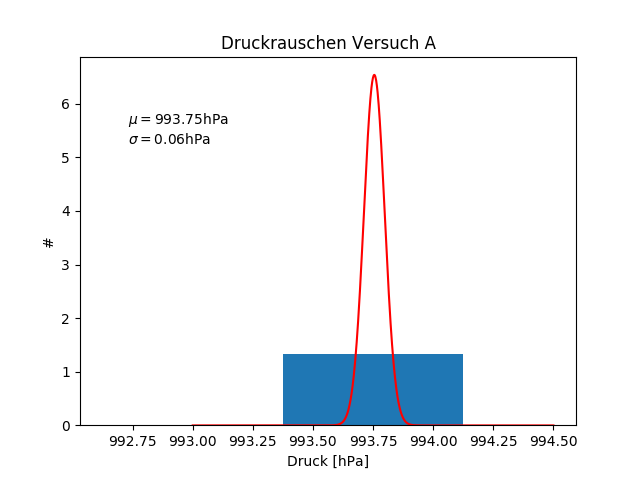
\includegraphics[scale=0.5]{Bilder/DruckrauschenA}
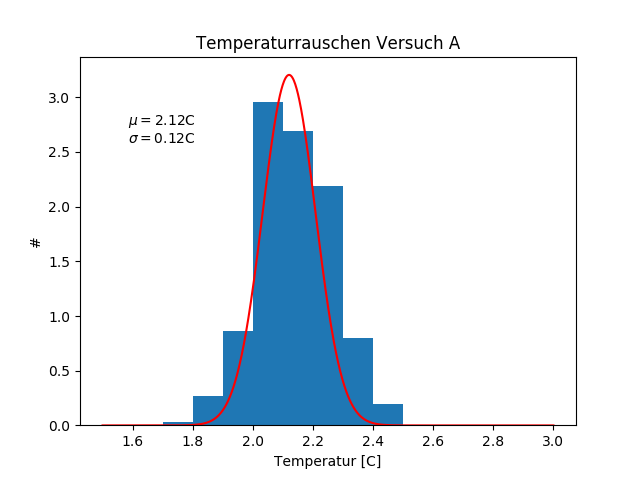
\includegraphics[scale=0.5]{Bilder/TemprauschenA}
\caption[Rauschen Versuch A]{Rauschmessung des Drucksensors (links) und des Temperaturfühlers (rechts). Eine Gaußkurve mit entsprechenden Parametern ist zusätzlich eingezeichnet.}
\label{fig:RauschenA}
\end{figure}

\begin{table}
\begin{center}
\begin{tabular}{|c|c|c|}
\hline
- & $\mu$ & $\sigma$\\
\hline
Druck & 993.75 & 0.006\\
\hline
Temperatur & 2.12 & 0.12\\
\hline
\end{tabular}
\caption[Tab. Rauschen A]{Ergebnisse der Rauschmessungen für Versuch A}
\label{tab:RauschenA}
\end{center}
\end{table}

Die Ergebnisse der Rauschmessungen sind in Abb. \ref{fig:RauschenA} und Tab. \ref{tab:RauschenA} dargestellt.

\subsubsection{Kalibrierung des Temperatursensors}
Bei jeweils 0C und 100C wurde eine Rauschmessung der Temperatur durchgeführt. Die Ergebnisse sind in Tabelle \ref{tab:KaliA} aufgeführt.

\begin{table}[H]
\begin{center}
\begin{tabular}{|c|c|}
\hline 
$T_{erwartet}[C]$ & $T_{gemessen}[C]$ \\ 
\hline 
$0$ & $2.12\pm0.12$ \\ 
\hline 
$100$ & $99.39\pm0.14$ \\ 
\hline 
\end{tabular}
\caption[Ergebnisse Kalibrierung A]{Ergebnisse Kalibrierung A} 
\label{tab:KaliA}
\end{center}
\end{table}

Aus diesen Ergebnissen wird nun eine Ausgleichsgerade bestimmt:

\begin{figure}[H]
\begin{center}
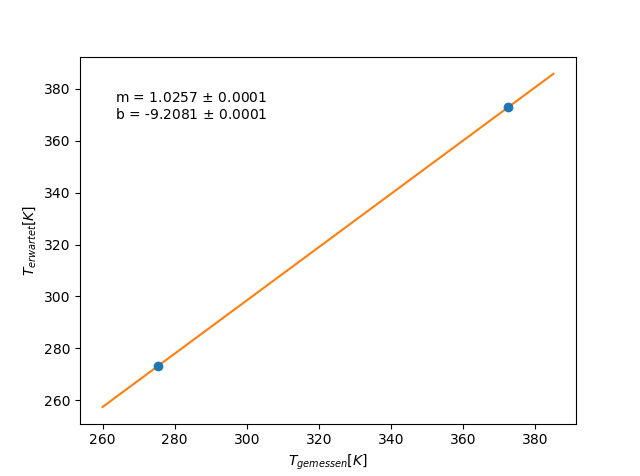
\includegraphics[width=\linewidth]{Bilder/KalibrationA}
\caption[Gerade Kalibration A]{Ausgleichsgerade bei der Kalibration(VersuchA)\\
Anmerkung: Die Fehler auf den Messungen sind sehr klein und deswegen hier nicht sichtbar.}
\label{fig:GeradeKaliA}
\end{center}
\end{figure}


Die Kalibrierung (Abb.\ref{fig:GeradeKaliA}) hat eine Steigung von $1.028\pm 0.002$ und einen Offset von $-2.1801\pm 0.005$.\\
Damit können die wirklichen Temperaturen berechnet werden:
\begin{equation}
T_{erwartet}=1.028\cdot T_{gemessen}-2.1801C
\end{equation}

Aus der Fehlerfortpflanzung folgt der Fehler auf die Temperatur:
\begin{equation}
\sigma_{T}=\sqrt{\sigma_{m}^{2}+\sigma_{b}^{2}}=0.005
\end{equation}
Dieser Fehler ist so klein, dass man ihn ignorieren kann.

\subsubsection{Dichtigkeitsmessung}
Eine sehr wichtige Voraussetzung für sinnvolle Ergebnisse ist, dass die Messapparatur dicht ist. Die Daten aus dem in Abschnitt \ref{sec:Aufbau und Durchfühung} erklärten Messverfahren vor dem Hauptversuch sind in Abbildung \ref{fig:DichtigkeitA} und die zugehörigen Residuen in Abbildung \ref{fig:ResiduenDichtigkeitA} zu sehen. Das Muster, dass sich in den Residuen zeigt, ist bedingt durch das Auflösungsvermögen des Drucksensor, welches eindrucksvoll anhand der Stufenform des Plots der Rohdaten zu sehen ist. \\
Aufgrund der Leckrate von $(0,215 \pm 0,02) \dfrac{hPa}{min}$ kann die Apparatur als dicht angenommen werden und der gemessene Druck kann direkt verwendet werden und muss nicht korrigiert werden.

\begin{figure}[H]
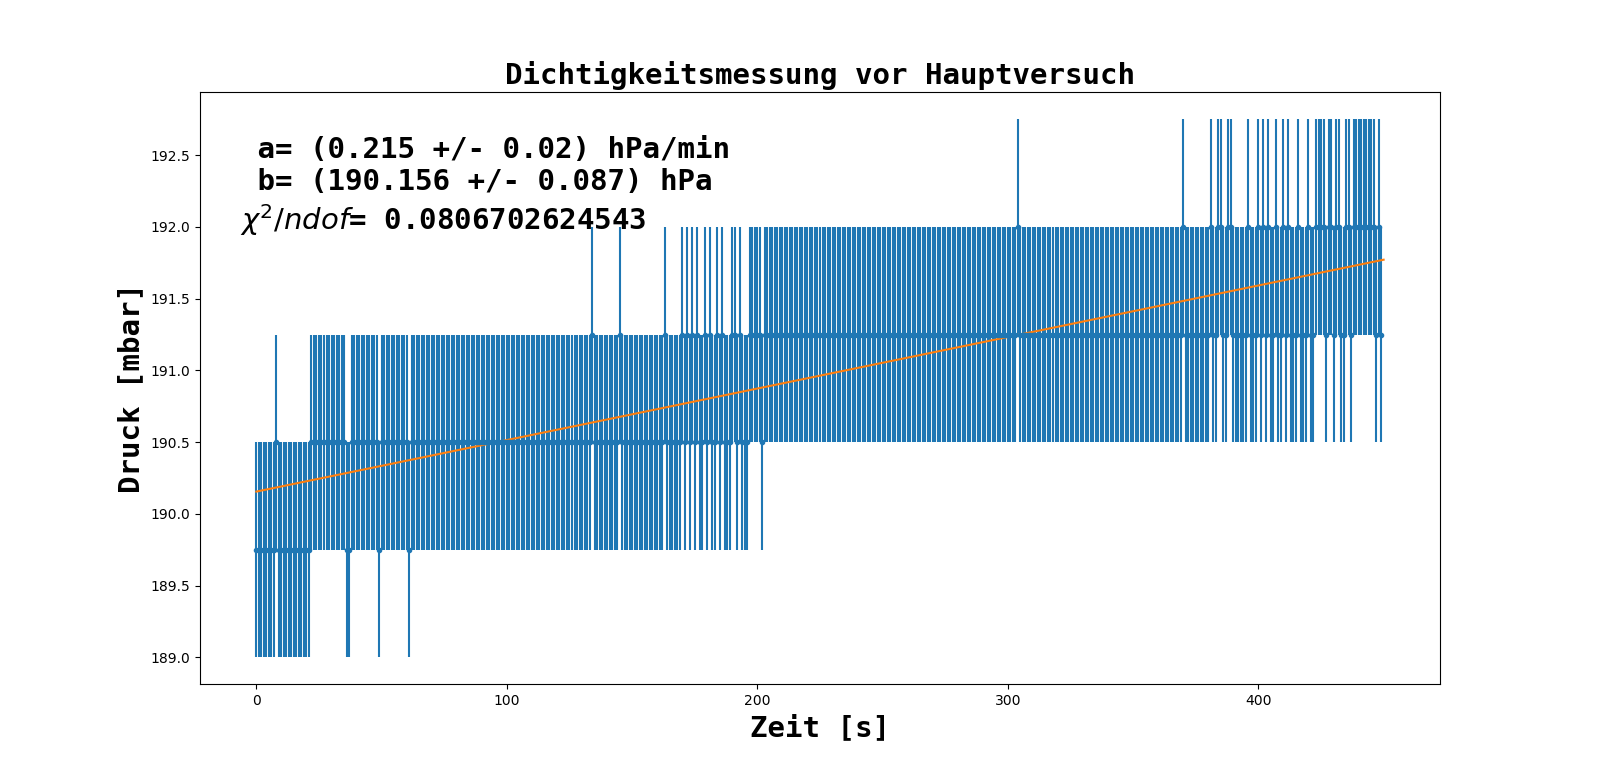
\includegraphics[width=\linewidth]{Bilder/Dichtigkeit_vorher_A.png}
\caption[Dichtigkeit vor Hauptversuch Apparatur A]{Dichtigkeit vor Hauptversuch Apparatur A}
\label{fig:DichtigkeitA}
\end{figure}

\begin{figure}[H]
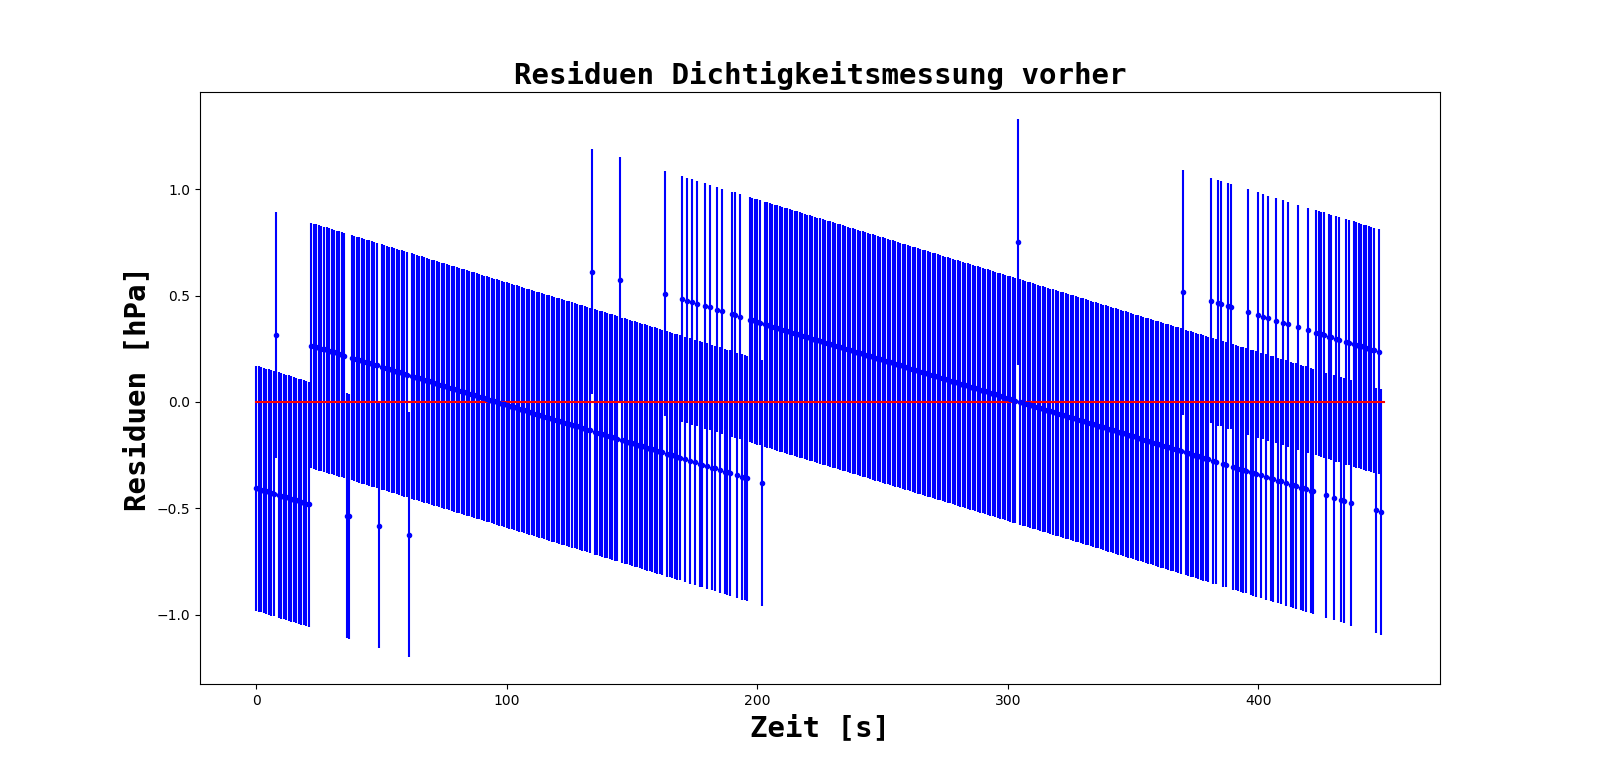
\includegraphics[width=\linewidth]{Bilder/Residuen_Dichtigkeit_vorher_A.png}
\caption[Dichtigkeit vor Hauptversuch Apparatur A]{Residuen der Dichtigkeit vor Hauptversuch Apparatur A}
\label{fig:ResiduenDichtigkeitA}
\end{figure}

\subsubsection{Auswertung}

\begin{figure}[H]
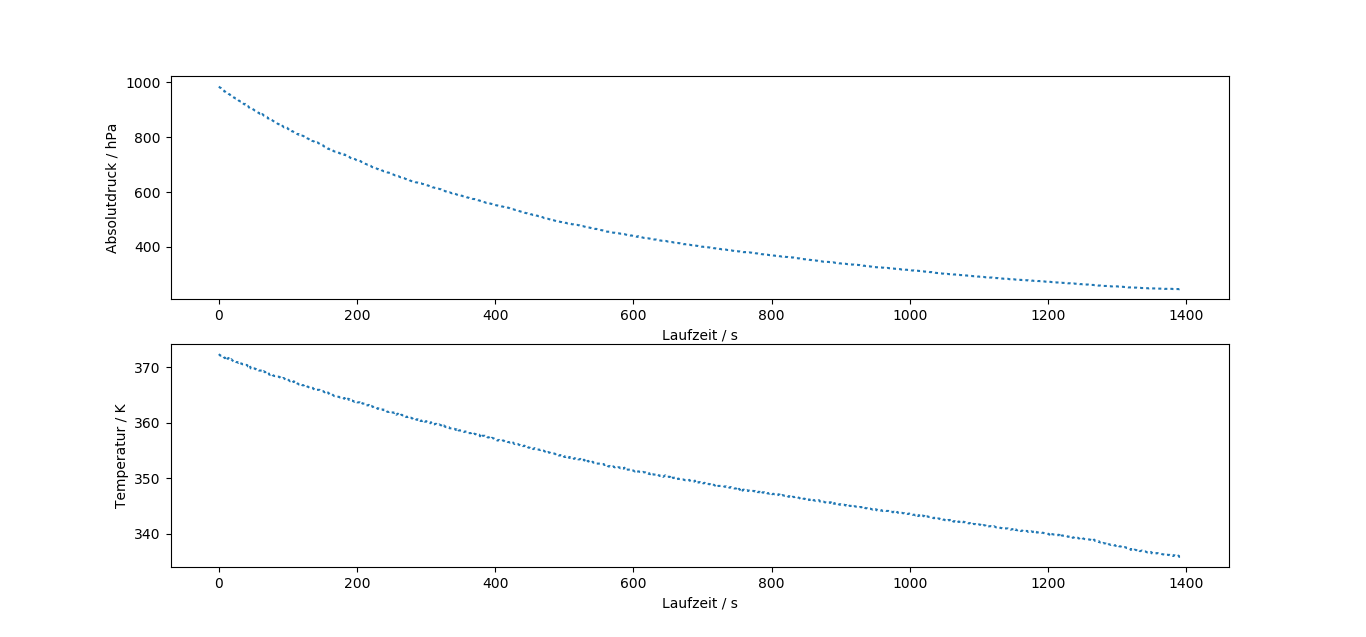
\includegraphics[width=\linewidth]{Bilder/Rohdaten_HauptmessungA.png}
\caption[Dichtigkeit vor Hauptversuch Apparatur A]{Druck und Temperatur im Verlauf der Messung}
\label{fig:RohdatenA}
\end{figure}

Die Rohdaten für Druck- und die Temperaturverlauf über die Zeit finden sich in Abbildung \ref{fig:RohdatenA}. Fügt man diese Daten über die Zeiten zusammen erhält man die Dampfdruckkurve (siehe Abbildung \ref{fig:DampfA}).\\

\begin{figure}[H]
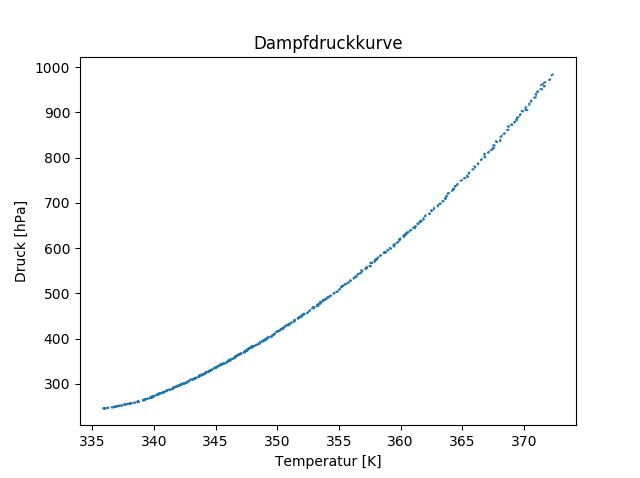
\includegraphics[scale=0.9]{Bilder/DampfdruckkurveA.png}
\caption[Dampfdruckkurve A]{Dampfdruckkurve in Versuch A}
\label{fig:DampfA}
\end{figure}

Der Fehler auf die Druckmessung ist gegeben durch die Digitalisierung und den Fehler der Rauschmessung:

\begin{equation}
\sigma_p=\sqrt{\left(\frac{0.75 hPa}{\sqrt{12}}\right)^2+(0.006 hPa)^2}=0.22 hPa
\end{equation}

Der Fehler auf die Temperaturmessung wird maßgeblich durch das Rauschen dominiert und ist damit gegeben durch $\sigma_T=0.12C$.\\
Trägt man nun den logarithmierten Druck gegen den Kehrwert der Temperatur auf, lässt sich der (lokale) lineare Zusammenhang gut erkennen(vgl. Abbildung \ref{fig:logA}).\\
Dabei ergeben sich die Fehler der transformierten Daten durch Fehlerfortpflanzung:

\begin{equation}
\sigma_{log(p/p_0}=\frac{\sigma_p}{p} ; \quad \sigma_{1/T}=\frac{\sigma_T}{T^2}
\end{equation}

Für den in Abbildung \ref{fig:logA} markierten Bereich ist die lineare Anpassung in Abbildung \ref{fig:fit_2A} exemplarisch gezeigt.\\

\begin{figure}[H]
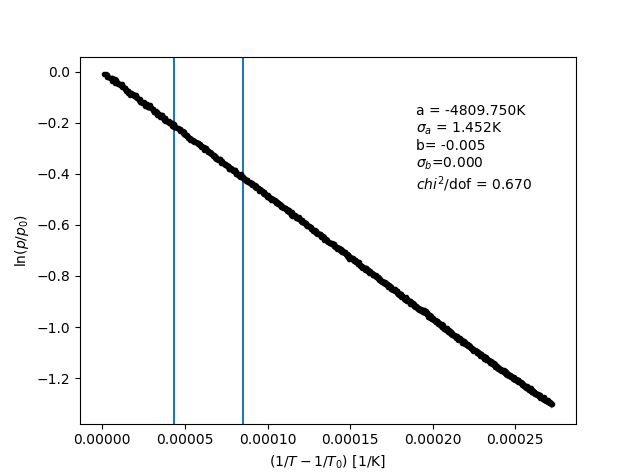
\includegraphics[width=\linewidth]{Bilder/log_RohdatenA.png}
\caption[Transformierte Daten A]{Transformierte Rohdaten für Versuch A}
\label{fig:logA}
\end{figure}

\begin{figure}
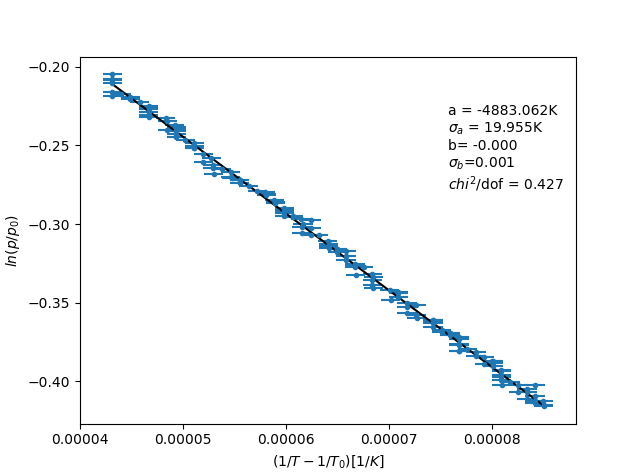
\includegraphics[width=\linewidth]{Bilder/lokaler_fit_2A.png}
\includegraphics[width=\linewidth]{Bilder/lokale_Residuen_2A}
\caption[Lokale Anpassung]{Lokale Anpassung im markierten Bereich und Residuen}
\label{fig:fit_2A}
\end{figure}
\newpage
Dieses Vorgehen wurde für insgesamt sechs, symmetrisch um eine bestimmte Temperatur verteilte, Teilintervalle durchgeführt. Die jeweiligen Ergebnisse sind in Tabelle \ref{tab:enthalpie_A}
aufgeführt.\\

\begin{table}[H]
	\begin{tabular}{|c|c|c|c|c|c|}
		\hline
		\textbf{Temp. [K]} & \textbf{Steigung fit [K]} & \textbf{y-Achsenabschn.} & $\chi ^2/dof$ & \textbf{$\Lambda$ [kJ/mol]} & \textbf{Abweichung} \\
		\hline
		373 & -5050.70 $\pm$ 16.62 & -0.266 $\pm$ 0.001 & 5.23 & 41.992 $\pm$ 0.138 & 9.6$\sigma$ \\
		\hline
		366 & -4989.34 $\pm$ 17.64 & -0.267 $\pm$ 0.001 & 3.59 & 41.481 $\pm$ 0.147 & 3.7$\sigma$ \\
		\hline
		361 & -4984.58 $\pm$ 19.38 & -0.269 $\pm$ 0.002 & 3.16 & 41.442 $\pm$ 0.161 & 1.6$\sigma$ \\
		\hline
		357 & -4954.29 $\pm$ 24.25 & -0.274 $\pm$ 0.003 & 2.65 & 41.190 $\pm$ 0.202 & 0.8$\sigma$ \\
		\hline
		353 & -5078.28 $\pm$ 26.35 & -0.258 $\pm$ 0.004 & 2.23 & 42.221 $\pm$ 0.219 & 3.3$\sigma$ \\
		\hline
		350 & -4736.43 $\pm$ 25.14 & -0.314 $\pm$ 0.004 & 1.90 & 39.379 $\pm$ 0.209 & 10$\sigma$ \\
		\hline 
	\end{tabular}
	\caption{Ergebnisse für die Verdampfungsenthalpie nach Temperatur (Mittelwert der Intervalle)}
	\label{tab:enthalpie_A}
\end{table}

Die Verdampfungsenthalpie ist dabei gegeben durch $\Lambda=-a \cdot R$ und der Fehler ergibt sich mittels Fehlerfortpflanzung zu $\sigma_{\Lambda}=R \cdot \sigma_a$.\\
Da $\Lambda$ temperaturabhängig ist, muss der zur Messung passende Literaturwert erst noch bestimmt werden. Da die Literaturwerte nicht trivial von der Temperatur abhängen, lassen sich diese nicht konkret ausrechnen. Abbildung \ref{fig:LiteraturwertLambda} zeigt die Literaturwerte als blaue Punkte und eine lineare Näherung als rote Linie. Es lässt sich leicht erkennen, dass die Näherung in diesem Temperaturbereich gut funktioniert. Daher wird mit dieser gerechnet und diese ist auch in die Ergebnisplots eingezeichnet. \\
In Abb. \ref{fig:EntTempA} findet sich die Auftragung der verschiedenen Werte von $\Lambda$ bei den entsprechenden Temperaturen.


\begin{figure}[H]
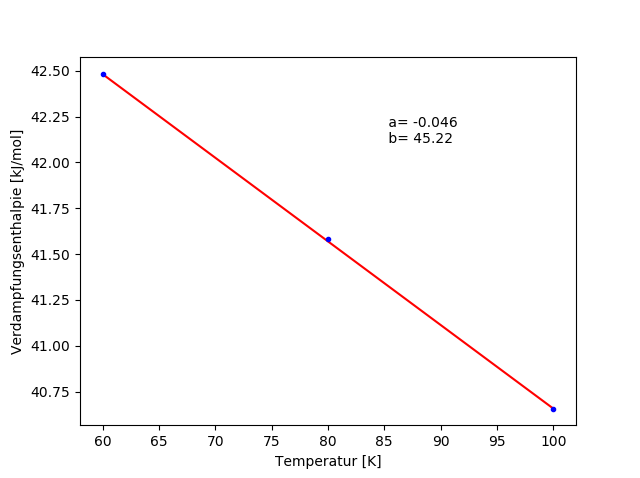
\includegraphics[scale=0.9]{Bilder/Lambda_Literaturwert_fit.png}
\caption[Literaturwerte für $\Lambda$ in Abhängigkeit von der Temperatur]{Literaturwerte für $\Lambda$ in Abhängigkeit von der Temperatur}
\label{fig:LiteraturwertLambda}
\end{figure}


\begin{figure}
\begin{center}
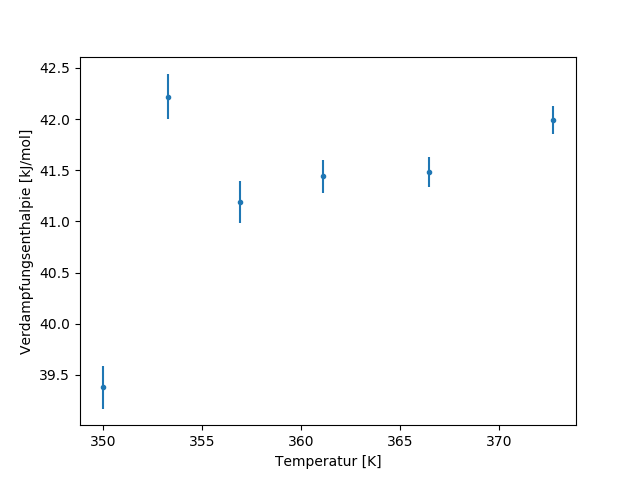
\includegraphics[scale=0.9]{Bilder/Enthalpie_gegen_TempA}
\caption{Enthalpie gegen Temperatur und Literaturwerte (Gerade).}
\label{fig:EntTempA}
\end{center}
\end{figure}

Es ist deutlich zu erkennen, dass die gemessenen Werte stark und ohne erkennbare Regelmäßigkeit von den Literaturwerten abweichen. 

\newpage
\subsection{Versuch B}


\subsubsection{Rauschmessung}

\begin{figure}[H]
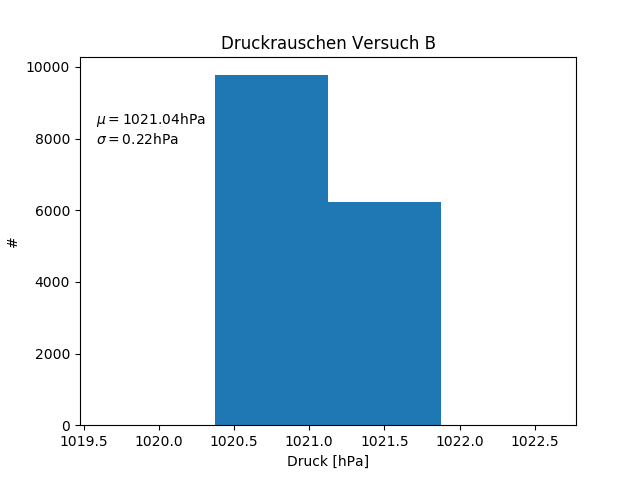
\includegraphics[scale=0.5]{Bilder/DruckrauschenB}
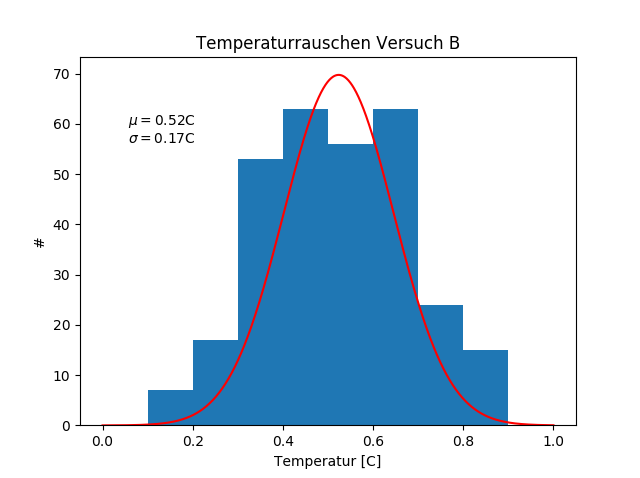
\includegraphics[scale=0.5]{Bilder/TemprauschenB}
\caption[Rauschmessung Versuch B]{Rauschmessung des Drucksensors (links) und des Temperaturfühlers (rechts)}
\label{fig:RauschenB}
\end{figure}

\begin{table}[H]
\begin{center}
\begin{tabular}{|c|c|c|}
\hline 
- & $\mu$ & $\sigma$\\ 
\hline 
Temperatur[C] & 22.99 & 0.04 \\ 
\hline 
Druck[hPa] & 1021.04 & 0.37\\ 
\hline 
\end{tabular}
\caption[Tabelle Rauschenmessung B]{Ergbenisse der Rauschmessung für Versuch B}
\label{tab:RauschenB}
\end{center}
\end{table}

Die Ergebnisse der Rauschmessungen für Versuch B finden sich in Abb. \ref{fig:RauschenB} und Tab. \ref{tab:RauschenB}.



\subsubsection{Kalibrierung des Temperatursensors}
Bei jeweils 0C und 100C wurde eine Rauschmessung der Temperatur durchgeführt. Die Ergebnisse sind in Tabelle \ref{tab:KaliB} dargestellt.

\begin{table}[H]
\begin{center}
\begin{tabular}{|c|c|}
\hline 
$T_{erwartet}[C]$ & $T_{gemessen}[C]$ \\ 
\hline 
0 & $0.52 \pm 0.17$ \\ 
\hline 
100 & $99.24\pm 0.09$ \\ 
\hline 
\end{tabular}
\caption[Ergebnisse Kalibrierung B]{Ergebnisse Kalibrierung B}
\label{tab:KaliB}
\end{center}
\end{table}
Aus diesen Ergebnissen wird nun eine Ausgleichsgerade bestimmt. (vgl. Abb. \ref{fig:GeradeKaliB})

\begin{figure}[H]
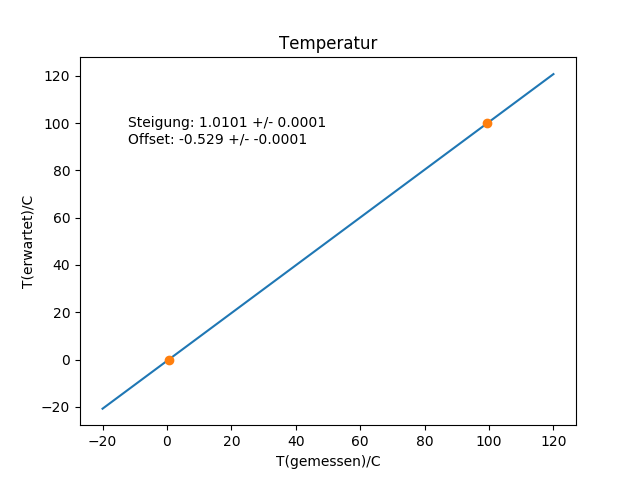
\includegraphics[width=\linewidth]{Bilder/KalibrationB}
\begin{center}
\caption[KalibrationB]{Ausgleichsgerade bei der Kalibration (VersuchB)\\
Anm.: Die Fehler auf den Messungen sind sehr klein und deswegen hier nicht sichtbar.}
\label{fig:GeradeKaliB}
\end{center}
\end{figure}

Die Kalibrierung hat eine Steigung von $1.013\pm 0.002$ und einen Offset von $-0.5304\pm 0.001$.\\
Damit können die wirklichen Temperaturen berechnet werden:
\begin{equation}
T_{erwartet}=1.013\cdot T_{gemessen}-0.5304
\end{equation}

Aus der Fehlerfortpflanzung folgt der Fehler auf die Temperatur:
\begin{equation}
\sigma_{T}=\sqrt{\sigma_{m}^{2}+\sigma_{b}^{2}}=0.002
\end{equation}
Dieser Fehler ist so klein, dass man ihn ignorieren kann.

\subsubsection{Dichtigkeitsmessung}
Die Daten aus dem in Abschnitt \ref{sec:Aufbau und Durchfühung} erklärten Messverfahren vor dem Hauptversuch sind in Abbildung \ref{fig:DichtigkeitB} und die zugehörigen Residuen in Abbildung \ref{fig:ResiduenDichtigkeitB} zu sehen. Das Muster, dass sich in den Residuen zeigt, ist bedingt durch das Auflösungsvermögen des Drucksensor, welches eindrucksvoll anhand der Stufenform des Plots der Rohdaten zu sehen ist. \\
Aufgrund der Leckrate von $(0,236 \pm 0,035) \dfrac{hPa}{min}$ kann die Apparatur als dicht angenommen werden und der gemessene Druck kann direkt verwendet werden und muss nicht korrigiert werden.\\
\\Für die Apparatur wurde noch eine zweite Dichtigkeitsmessung nach dem Hauptversuch durchgeführt. Die Daten sind in Abbildung \ref{fig:DichtigkeitNachherB} und die zugehörigen Residuen in Abbildung \ref{fig:ResiduenDichtigkeitNachherB}.\\
Die Leckrate ist mit $(2,718 \pm 0,160) \dfrac{hPa}{min}$ deutlich schlechter geworden im Vergleich zu der Leckrate vor dem Hauptversuch. Dies könnte daran liegen, dass die Dichtigkeitsmessung nicht mit dem nach dem Hauptversuch vorhandenen Unterdruck durchgeführt wurde, sondern wie zu Beginn mit der Handvakuumpumpe. Durch das Wackeln an der Apparatur beim Anschließen dieser könnten sich Undichtigkeiten aufgetan haben, welche dann den Wert der zweiten Messung verschlechtert haben, auf die Hauptmessung aber keinen Einfluss haben, weil sie erst nach dieser aufgetreten sind. Daher wird im Folgenden davon dennoch ausgegangen, dass die Undichtigkeit vernachlässigbar gering ist.

\begin{figure}[H]
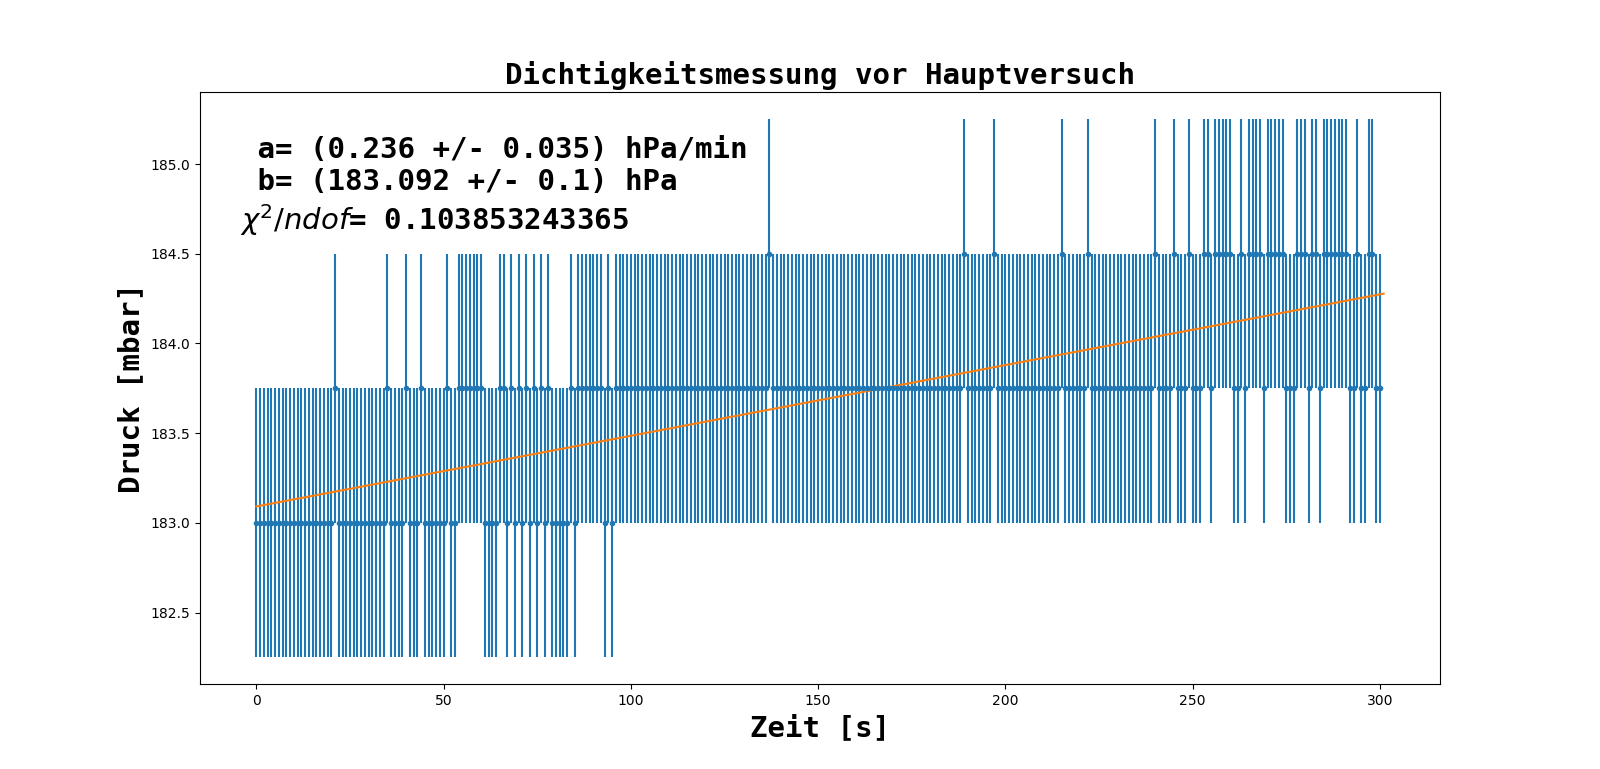
\includegraphics[width=\linewidth]{Bilder/Dichtigkeit_vorher_B.png}
\caption[Dichtigkeit vor Hauptversuch Apparatur B]{Dichtigkeit vor Hauptversuch Apparatur B}
\label{fig:DichtigkeitB}
\end{figure}

\begin{figure}[H]
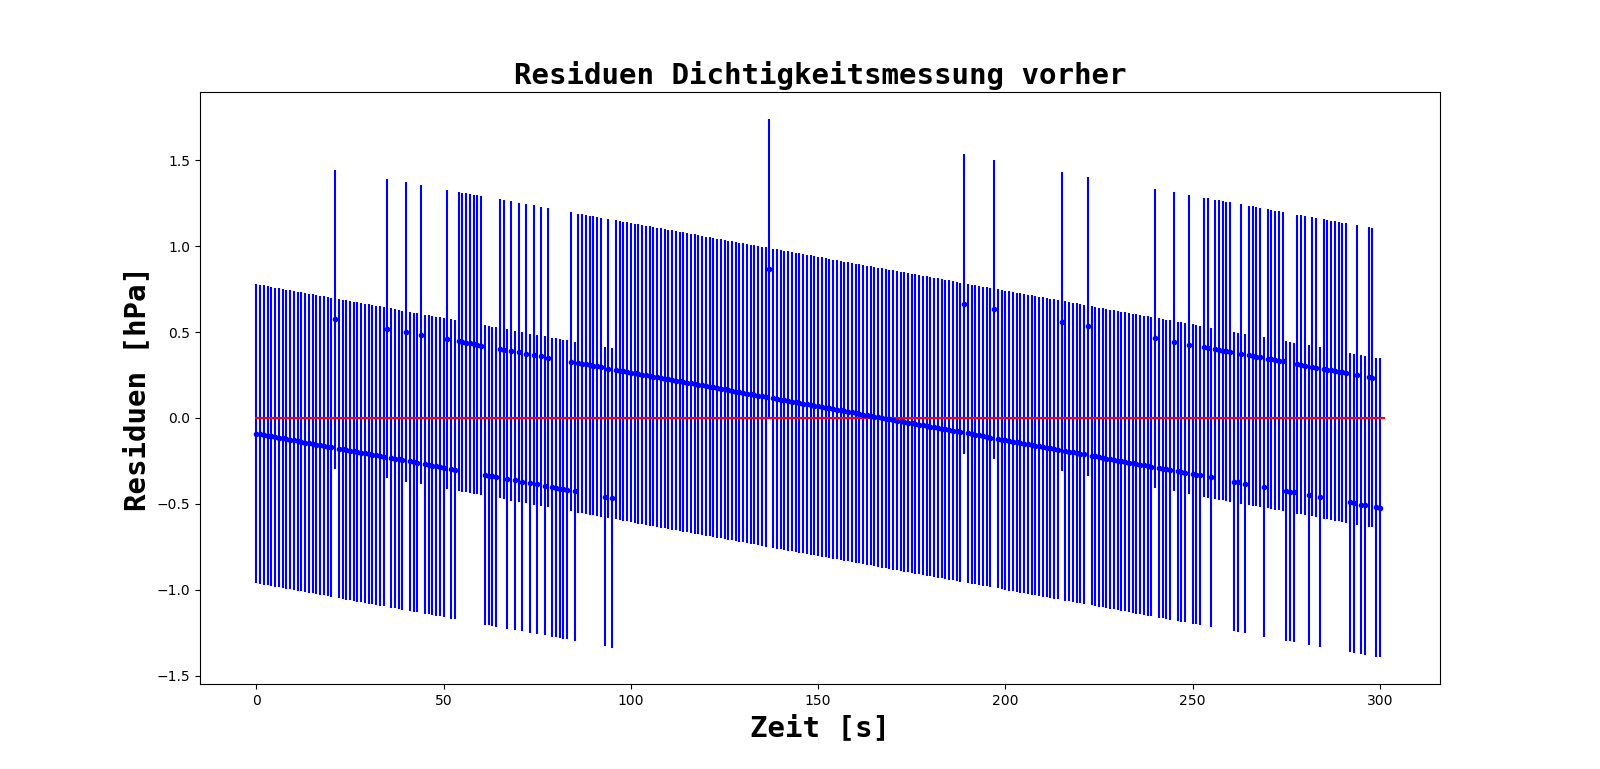
\includegraphics[width=\linewidth]{Bilder/Residuen_Dichtigkeit_vorher_B.png}
\caption[Dichtigkeit vor Hauptversuch Apparatur B]{Residuen der Dichtigkeit vor Hauptversuch Apparatur B}
\label{fig:ResiduenDichtigkeitB}
\end{figure}

\begin{figure}[H]
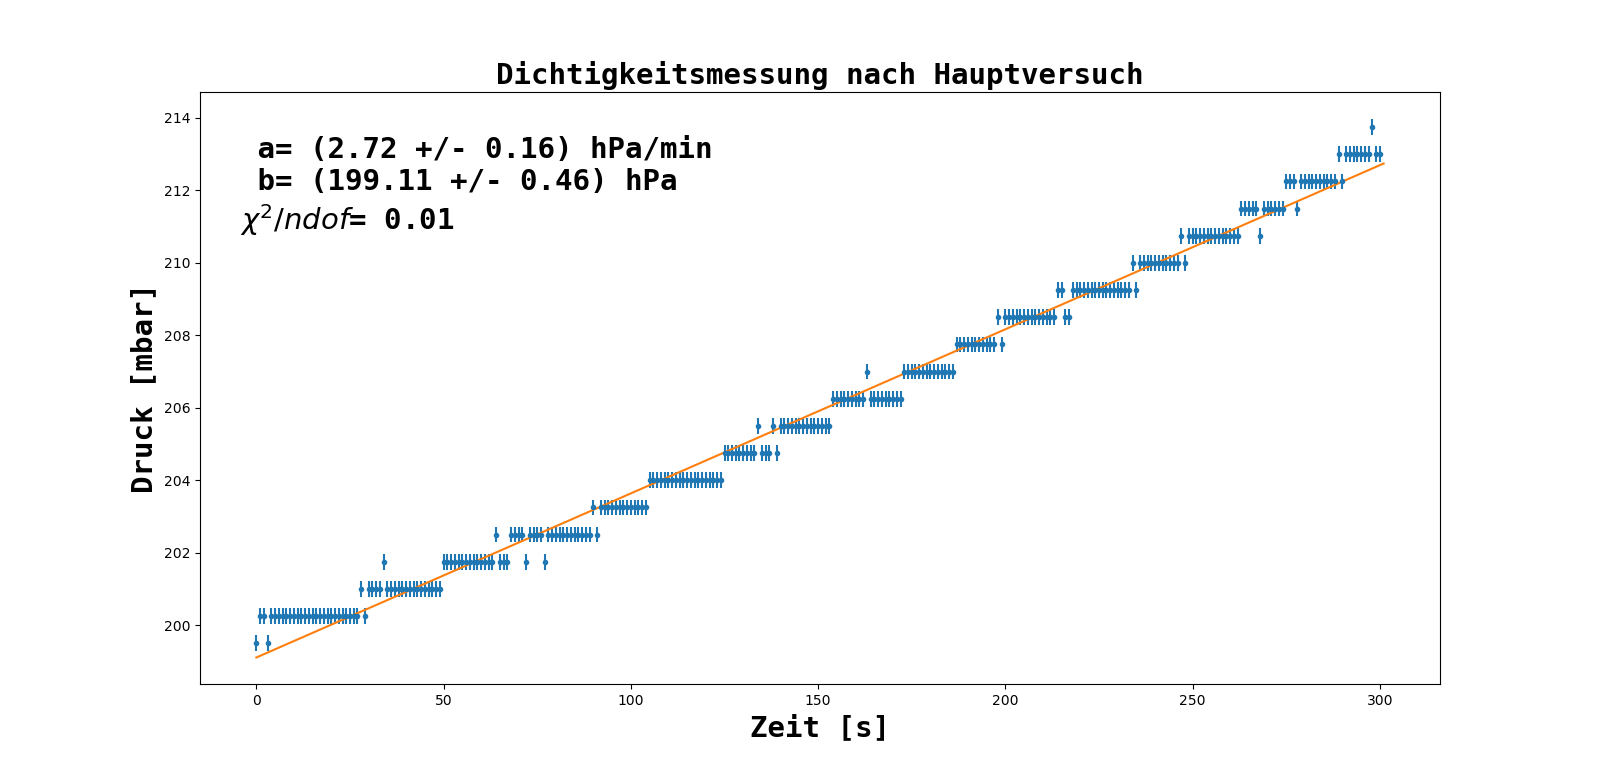
\includegraphics[width=\linewidth]{Bilder/Dichtigkeit_nachher_B.png}
\caption[Dichtigkeit vor Hauptversuch Apparatur B]{Dichtigkeit nach Hauptversuch Apparatur B}
\label{fig:DichtigkeitNachherB}
\end{figure}

\begin{figure}[H]
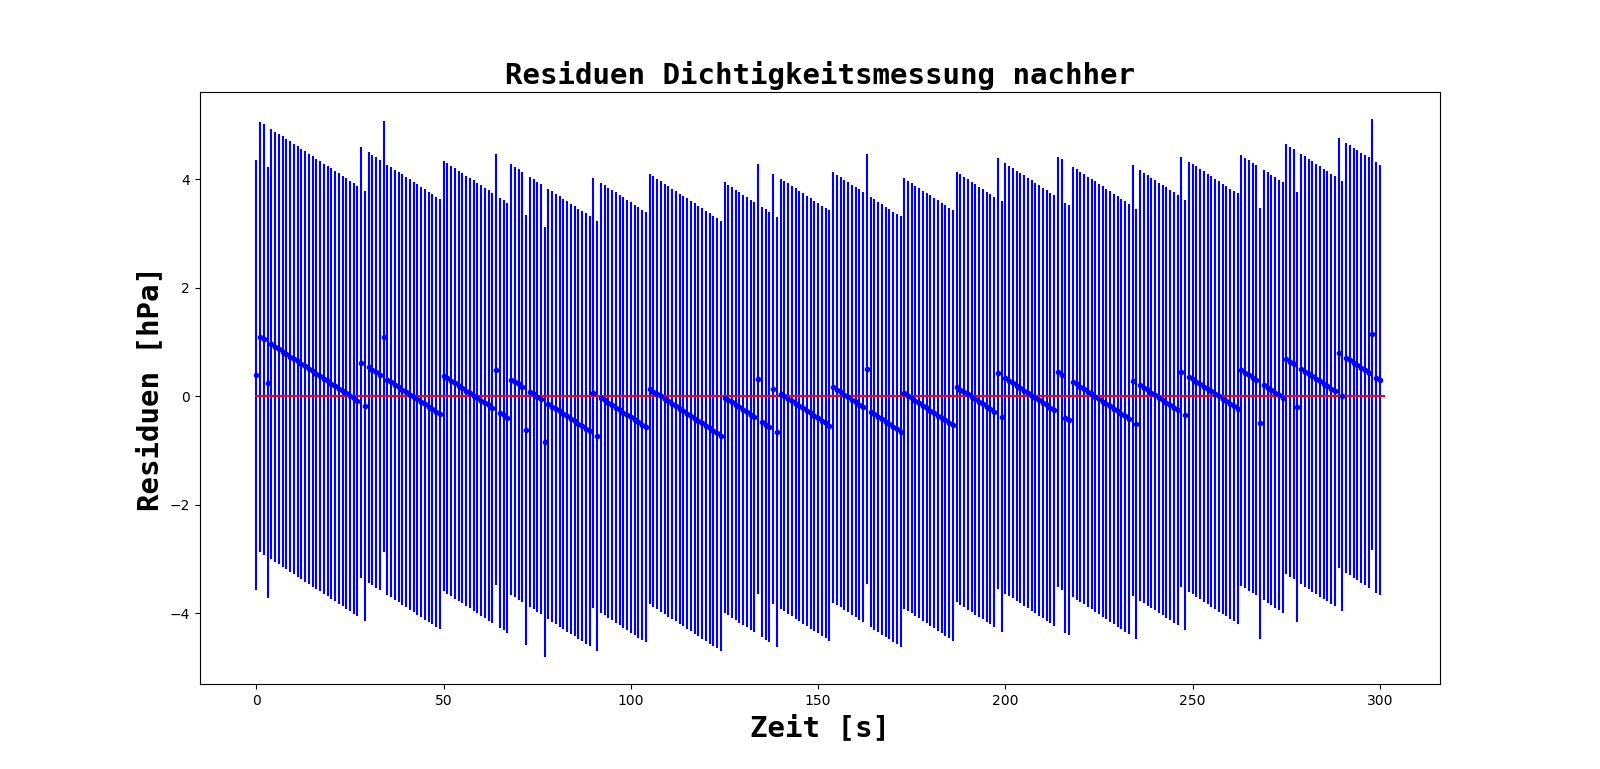
\includegraphics[width=\linewidth]{Bilder/Residuen_Dichtigkeit_nachher_B.png}
\caption[Dichtigkeit nach Hauptversuch Apparatur B]{Residuen der Dichtigkeit nach Hauptversuch Apparatur B}
\label{fig:ResiduenDichtigkeitNachherB}
\end{figure}

\newpage
\subsubsection{Auswertung}

Eine Aufzeichnung von Druck und Temperatur im Verlauf der Messung findet sich in Abb. \ref{fig:RohdatenB}. Die sich daraus ergebende Dampfdruckkurve ist in Abb.\ref{fig:DampfB} dargestellt.\\

\begin{figure}[H]
\begin{center}
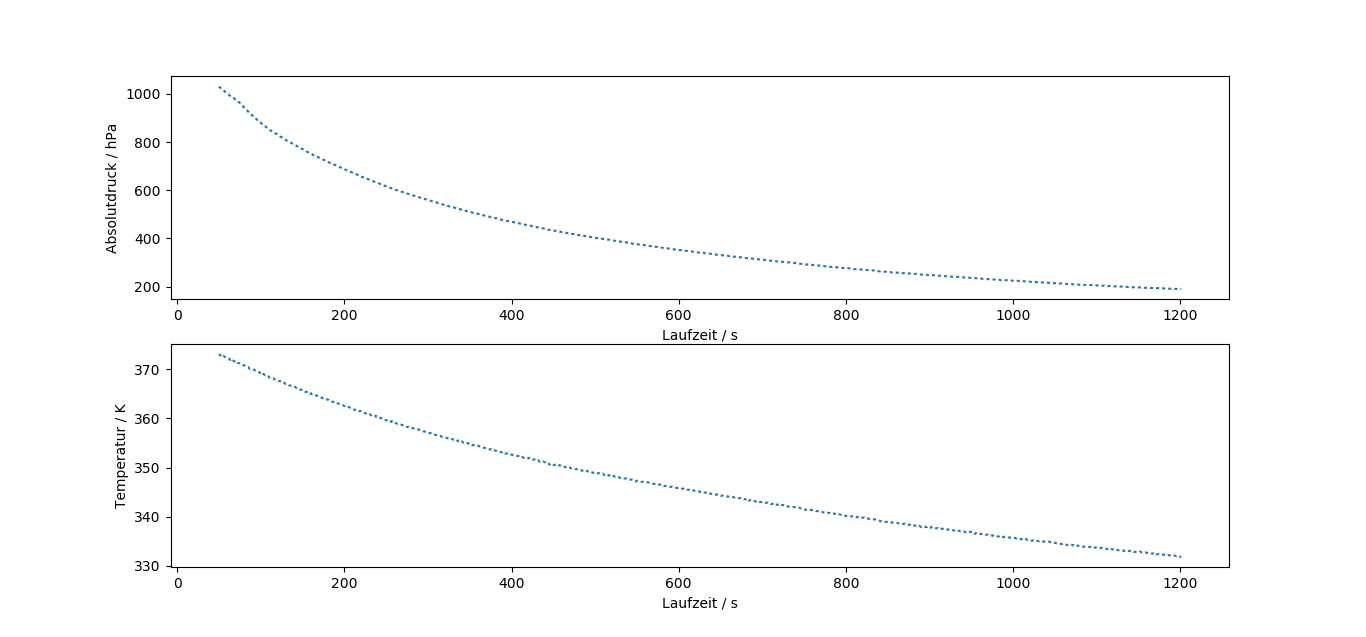
\includegraphics[scale=0.4]{Bilder/Rohdaten_HauptmessungB}
\caption[Rohdaten B]{Druck und Temperatur im Verlauf der Messung.}
\label{fig:RohdatenB}
\end{center}
\end{figure}

\begin{figure}[H]
\begin{center}
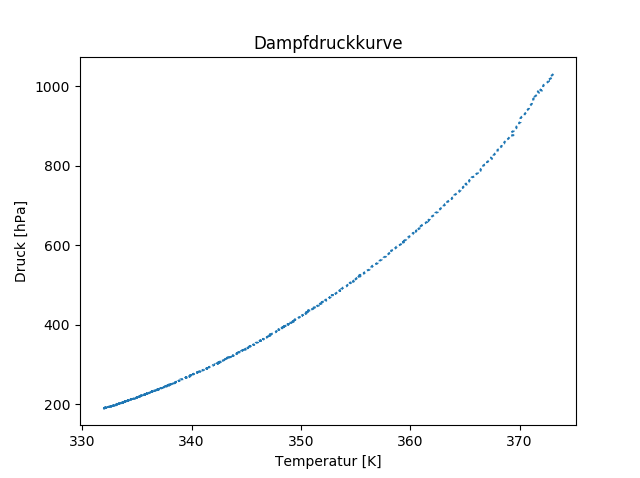
\includegraphics[scale=0.8]{Bilder/DampfdruckkurveB}
\caption[Dampfdruckkurve B]{Dampfdruckkurve in Versuch B.}
\label{fig:DampfB}
\end{center}
\end{figure}
\newpage
Bei entsprechender Transformation der Messwerte (erfolgt durch direkte Aufzeichnung mittels CASSY und der Funktion \glqq Größe definieren \grqq) ist bereits deutlich der zumindest lokal gültige lineare Zusammenhang erkennbar (Abb.\ref{fig:logB}).

\begin{figure}[H]
\begin{center}
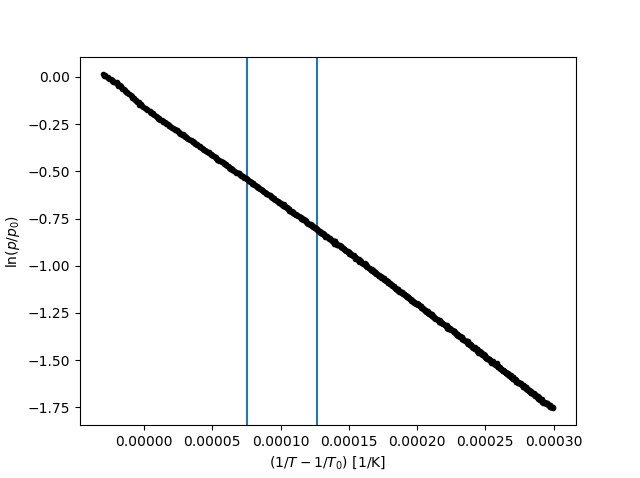
\includegraphics[width=\linewidth]{Bilder/log_RohdatenB}
\caption[Rohdaten logarith. B]{Transformierte Rohdaten}
\label{fig:logB}
\end{center}
\end{figure}

Für den markierten Bereich in der transformierten Darstellung ist die lokale Anpassung exemplarisch in Abb.\ref{fig:fit_2B} durchgeführt worden.\\
Weitere Anpassungen auf symmetrischen Intervallen bestimmter (reziproke) Temperaturwerte wurden durchgeführt. Die Ergebnisse finden sich in Tab. \ref{tab:enthalpie_B}.

\begin{table}[H]
	\begin{tabular}{|c|c|c|c|c|c|}
		\hline
		\textbf{Temp. [K]} & \textbf{Steigung fit [K]} & \textbf{y-Achsenabschn.} & $\chi ^2/dof$ & \textbf{$\Lambda$ [kJ/mol]} & \textbf{Abweichung} \\
		\hline
		367 & -5020.08 $\pm$ 9.44 & -0.165 $\pm$ 0.001 & 2.29 & 40.783 $\pm$ 0.076 & 1.9$\sigma$ \\
		\hline
		359 & -5156.11 $\pm$ 11.95 & -0.154 $\pm$ 0.001 & 1.75 & 41.559 $\pm$ 0.096 & 2.9$\sigma$ \\
		\hline
		353 & -5307.76 $\pm$ 21.64 & -0.135 $\pm$ 0.003 & 2.84 & 42.428 $\pm$ 0.172 & 5.3$\sigma$ \\
		\hline
		348 & -5425.55 $\pm$ 20.72 & -0.118 $\pm$ 0.004 & 1.55 & 42.995 $\pm$ 0.165 & 7.6$\sigma$ \\
		\hline
		344 & -5476.23 $\pm$ 24.03 & -0.108 $\pm$ 0.005 & 1.50 & 42.991 $\pm$ 0.188 & 5.8$\sigma$ \\
		\hline
		341 & -5654.39 $\pm$ 34.72 & -0.067 $\pm$ 0.009 & 1.72 & 43.932 $\pm$ 0.270 & 7.1$\sigma$ \\
		\hline
	\end{tabular}
	\caption{Ergebnisse für die Verdampfungsenthalpie nach Temperatur für Versuch B}
	\label{tab:enthalpie_B}
\end{table}

\begin{figure}[H]
\begin{center}
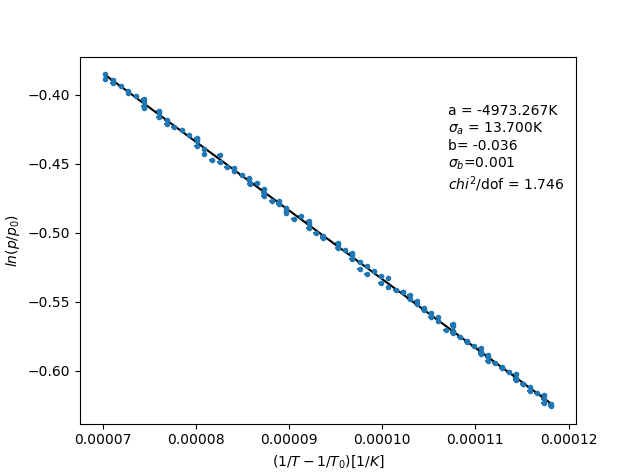
\includegraphics[width=\linewidth]{Bilder/lokaler_fit_2B}\\
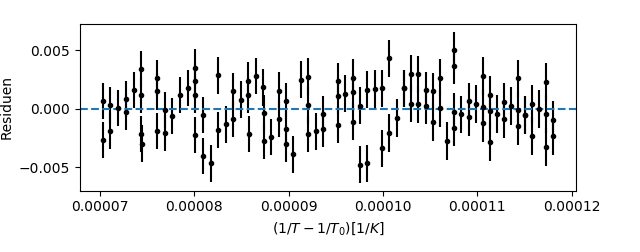
\includegraphics[width=\linewidth]{Bilder/lokale_residuen_2B}
\caption[Lokale Anpassung]{Lokale Anpassung im markierten Bereich und Residuen}
\label{fig:fit_2B}
\end{center}
\end{figure}





Die so erhaltenen Werte für die Verdampfungsenthalpie können gegen die dazugehörige Temperatur aufgetragen werden. Man erhält dann Abb.\ref{fig:EntTempB}.

\begin{figure}[H]
\begin{center}
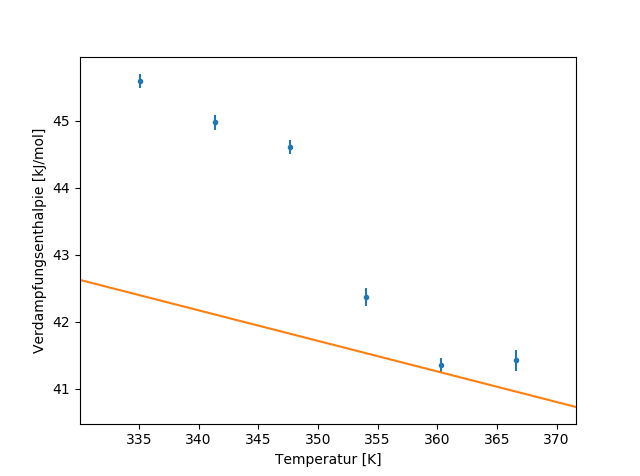
\includegraphics[scale=0.8]{Bilder/Enthalpie_gegen_TempB}
\caption[Enthalpie - Temperatur]{Errechnete Enthalpiewerte aufgetragen gegen die entsprechende Temperatur und Literaturwerte (Gerade).}
\label{fig:EntTempB}
\end{center}
\end{figure}

Es ist direkt ersichtlich, dass der prinzipielle Verlauf von Verdampfungsenthalpie gegen Temperatur mit dem Verlauf aus der Literatur übereinstimmt. Allerdings sind die individuellen Werte im Vergleich zu den Literaturwerten zum Teil mehrere Standardabweichungen zu groß, was dafür spricht, dass das Versuchsergebnis durch eine unerkannte Systematik stark nach oben verfälscht wird.\\
Denn ein zu großer Druck (z.B. durch den Partialdruck zusätzlich eingeschlossener Luft) sorgt für eine betragsmäßig größere Steigung und infolge dessen zu einem erhöhten Wert für $\Lambda$.
Ebenso ist klar erkennbar, dass die Abweichung mit zunehmender Messdauer (entspricht kleinerer Temperatur) immer mehr zunimmt. Berücksichtigt man noch die zweite Dichtigkeitsmessung, welche deutlich schlechter als die erste ausgefallen ist, lässt sich zusammenfassend sagen das während des Versuches eine ausreichend große Menge Luft in den Kolben eingedrungen ist und somit der gemessene Druck zunehmend größer als der tatsächliche Dampfdruck des Wassers wurde.


\end{document}
